\subsection{Minimale Anzahl Hinweise}
Die minimale Anzahl für ein eindeutig lösbares $9 \times 9$ Sudoku sind 17 Hinweise~\cite{DBLP:journals/corr/abs-1201-0749}.
Für $4 \times 4$ und $6 \times 6$ Sudokus haben wir alles Anordnungen an Hinweisen selbst getestet.
Für $4 \times 4$ Sudokus sind es 4 Hinweise und für $6 \times 6$ Sudokus sind es 8 Hinweise.
Jeweils ein Beispiel für diese minimalen Sudokus lassen sich in \cref{fig:minimal_hinweise} finden.


\begin{figure}[H]
    \centering
    \begin{minipage}{0.48\textwidth}
        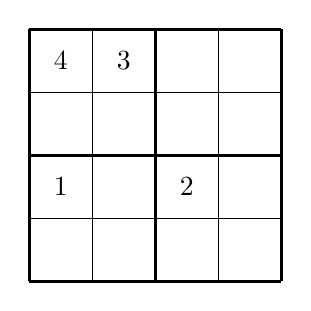
\begin{tikzpicture}
            % Zellgröße
            \def\s{0.8cm}

            % 4x4 Sudoku (Beispiel-Lösung, anpassbar)
            \def\sudoku{
                    {4,3, , },
                    { ,,,},
                    {1,, 2, },
                    { ,,,},
            }

            % Rasterlinien
            \foreach \x in {0,1,...,4} {
                \draw[thin] (\x*\s, 0) -- (\x*\s, 4*\s);
                \draw[thin] (0, \x*\s) -- (4*\s, \x*\s);
            }
            \foreach \x in {0,2,4} {
                \draw[very thick] (\x*\s, 0) -- (\x*\s, 4*\s);
                \draw[very thick] (0, \x*\s) -- (4*\s, \x*\s);
            }

            % Zahlen eintragen
            \foreach \row [count=\i from 0] in \sudoku {
                \foreach \num [count=\j from 0] in \row {
                    \node at (\j*\s + 0.5*\s, 3.5*\s - \i*\s) {\num};
                }
            }
        \end{tikzpicture}
    \end{minipage}
    \hfill
    \begin{minipage}{0.48\textwidth}
        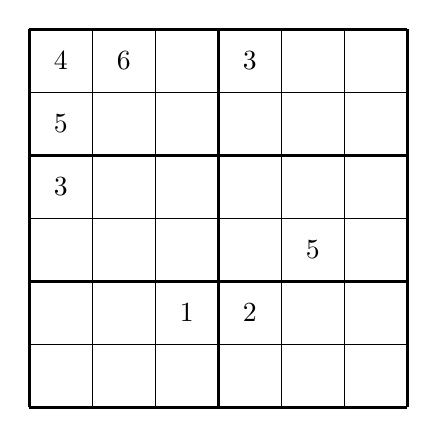
\begin{tikzpicture}
            % Zellgröße
            \def\s{0.8cm}

            % 6x6 Sudoku (Beispiel – anpassbar)
            \def\sudoku{
                    {4,6,,3,,},
                    {5,,,,,},
                    {3,,,,,},
                    {,,,,5,},
                    {,,1,2,,},
                    {,,,,,},
            }

            % Rasterlinien
            \foreach \x in {0,1,...,6} {
                \draw[thin] (\x*\s, 0) -- (\x*\s, 6*\s);
                \draw[thin] (0, \x*\s) -- (6*\s, \x*\s);
            }
            % Dicke Linien für 3-Spalten-Blöcke und 2-Zeilen-Blöcke
            \foreach \x in {0,3,6} {
                \draw[very thick] (\x*\s, 0) -- (\x*\s, 6*\s);
            }
            \foreach \y in {0,2,4,6} {
                \draw[very thick] (0, \y*\s) -- (6*\s, \y*\s);
            }

            % Zahlen eintragen
            \foreach \row [count=\i from 0] in \sudoku {
                \foreach \num [count=\j from 0] in \row {
                    \node at (\j*\s + 0.5*\s, 5.5*\s - \i*\s) {\num};
                }
            }
        \end{tikzpicture}
    \end{minipage}
    \caption{Beispiele für minimale Sudokus}
    \label{fig:minimal_hinweise}
\end{figure}





\subsection{Symmetrien}
Ein 9x9 Sudoku besteht aus 3 horizontalen und 3 vertikalen Bändern.
Die Bänder bestehen jeweils aus 3 Zeilen beziehungsweise 3 Spalten. \\
Die Tupel (1, 2, 3), (4, 5, 6), (7, 8, 9) beschreiben die Zeilen oder Spalten der jeweiligen Bänder. \\
Mit dem Wissen über die Bänder können wir die Symmetrien eines Sudokus formulieren~\cite{russell2006mathematics}: \\
\begin{itemize}
    \item Permutation der 9 Ziffern
    \item Permutation der 3 horizontalen Bänder
    \item Permutation der 3 vertikalen Bänder
    \item Permutation der Zeilen innerhalb eines horizontalen Bandes
    \item Permutation der Spalten innerhalb eines vertikalen Bandes
    \item Spiegelung und Rotation
\end{itemize}
Insgesamt gibt es in etwa 6,7 Trilliarden verschiedene valide Sudokus \cite{felgenhauer2006mathematics}.
Unter Berücksichtigung der Symmetrien gibt es ungefähr 5,5 Milliarden verschiedene valide Sudokus\cite{russell2006mathematics}. \\
Wir haben verschiedene Experimenter mit den Symmetrien durchgeführt, allerdings keine signifikanten Ergebnisse erzielt.
Deswegen haben wir im finalen Backend nur die Permutation der Ziffern verwendet.

\subsection{Anzahl Hinweise pro Band}

\begin{figure}[H]
    \centering
    \begin{minipage}{0.48\textwidth}
        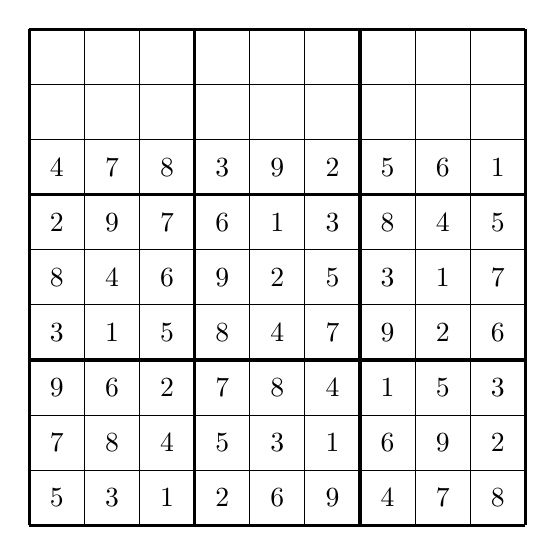
\begin{tikzpicture}
            % Zellgröße
            \def\s{0.7cm}

            % Sudoku-Lösung (kann beliebig angepasst werden)
            \def\sudoku{
                    {, , , , , , , , },
                    {, , , , , , , , },
                    {4, 7, 8, 3, 9, 2, 5, 6, 1},
                    {2, 9, 7, 6, 1, 3, 8, 4, 5},
                    {8, 4, 6, 9, 2, 5, 3, 1, 7},
                    {3, 1, 5, 8, 4, 7, 9, 2, 6},
                    {9, 6, 2, 7, 8, 4, 1, 5, 3},
                    {7, 8, 4, 5, 3, 1, 6, 9, 2},
                    {5, 3, 1, 2, 6, 9, 4, 7, 8},
            }

            % Rasterlinien
            \foreach \x in {0,1,...,9} {
                \draw[thin] (\x*\s, 0) -- (\x*\s, 9*\s);
                \draw[thin] (0, \x*\s) -- (9*\s, \x*\s);
            }
            \foreach \x in {0,3,6,9} {
                \draw[very thick] (\x*\s, 0) -- (\x*\s, 9*\s);
                \draw[very thick] (0, \x*\s) -- (9*\s, \x*\s);
            }




            % Zahlen eintragen
            \foreach \row [count=\i from 0] in \sudoku {
                \foreach \num [count=\j from 0] in \row {
                % Y-Koordinate: Startet oben bei 8.5 und geht pro Zeile 1 runter
                    \node at (\j*\s + 0.5*\s, 8.5*\s - \i*\s) {\num};
                }
            }
        \end{tikzpicture}
    \end{minipage}
    \hfill
    \begin{minipage}{0.48\textwidth}
        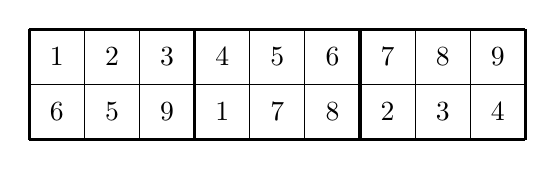
\begin{tikzpicture}[baseline]
            % Zellgröße
            \def\s{0.7cm}

            % Werte für das 2x9 Gitter
            \def\zweizeilen{
                    {1, 2, 3, 4, 5, 6, 7, 8, 9},
                    {6, 5, 9, 1, 7, 8, 2, 3, 4},
            }

            % Rasterlinien
            \foreach \x in {0,1,...,9} {
                \draw[thin] (\x*\s, 0) -- (\x*\s, 2*\s);
            }
            \foreach \y in {0,1,2} {
                \draw[thin] (0, \y*\s) -- (9*\s, \y*\s);
            }

            % Dickere Linien wie bei Sudoku
            \foreach \x in {0,3,6,9} {
                \draw[very thick] (\x*\s, 0) -- (\x*\s, 2*\s);
            }
            \draw[very thick] (0, 0) -- (9*\s, 0);
            \draw[very thick] (0, 2*\s) -- (9*\s, 2*\s);

            % Zahlen eintragen
            \foreach \row [count=\i from 0] in \zweizeilen {
                \foreach \num [count=\j from 0] in \row {
                    \node at (\j*\s + 0.5*\s, 1.5*\s - \i*\s) {\num};
                }
            }
        \end{tikzpicture}
        \\
        \\

        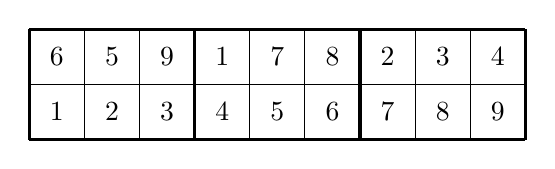
\begin{tikzpicture}[baseline]
            % Zellgröße
            \def\s{0.7cm}

            % Werte für das 2x9 Gitter
            \def\zweizeilen{
                    {6, 5, 9, 1, 7, 8, 2, 3, 4},
                    {1, 2, 3, 4, 5, 6, 7, 8, 9},
            }

            % Rasterlinien
            \foreach \x in {0,1,...,9} {
                \draw[thin] (\x*\s, 0) -- (\x*\s, 2*\s);
            }
            \foreach \y in {0,1,2} {
                \draw[thin] (0, \y*\s) -- (9*\s, \y*\s);
            }

            % Dickere Linien wie bei Sudoku
            \foreach \x in {0,3,6,9} {
                \draw[very thick] (\x*\s, 0) -- (\x*\s, 2*\s);
            }
            \draw[very thick] (0, 0) -- (9*\s, 0);
            \draw[very thick] (0, 2*\s) -- (9*\s, 2*\s);

            % Zahlen eintragen
            \foreach \row [count=\i from 0] in \zweizeilen {
                \foreach \num [count=\j from 0] in \row {
                    \node at (\j*\s + 0.5*\s, 1.5*\s - \i*\s) {\num};
                }
            }
        \end{tikzpicture}
    \end{minipage}
    \caption{Beispiel für Zeilenvertauschung}
    \label{fig:row_constraints}
\end{figure}

In einem partiellen Sudoku darf es in einem horizontalen Band keine zwei Zeilen ohne Hinweise geben.
In \cref{fig:row_constraints} kann man sehen, dass es ansonsten mehrere Lösungen gibt.
Obwohl alle Hinweise bis auf zwei komplette Zeilen gegeben sind, gibt es trotzdem zwei mögliche Lösungen.
Äquivalent dazu dürfen in einem vertikalen Band keine zwei Spalten ohne Hinweise sein.
Übersetzt man dies auf allgemeine Sudoku-Größen,
muss in einem Band der Breite beziehungsweise Höhe $n$ mindestens $n-1$ Spalten beziehungsweise Zeilen mit mindestens einem Hinweis gegeben sein.

\subsection{Unterquadrate}
\label{sec:unterquadrate}

\begin{figure}[H]
    \centering
    \begin{minipage}{0.48\textwidth}
            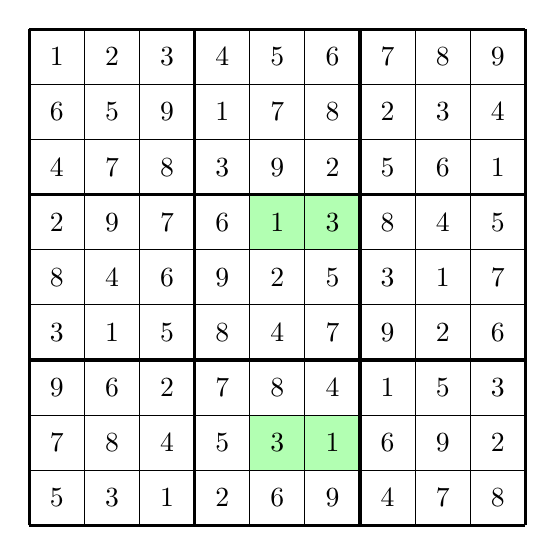
\begin{tikzpicture}
                % Zellgröße
                \def\s{0.7cm}

                % Sudoku-Lösung (kann beliebig angepasst werden)
                \def\sudoku{
                        {1, 2, 3, 4, 5, 6, 7, 8, 9},
                        {6, 5, 9, 1, 7, 8, 2, 3, 4},
                        {4, 7, 8, 3, 9, 2, 5, 6, 1},
                        {2, 9, 7, 6, 1, 3, 8, 4, 5},
                        {8, 4, 6, 9, 2, 5, 3, 1, 7},
                        {3, 1, 5, 8, 4, 7, 9, 2, 6},
                        {9, 6, 2, 7, 8, 4, 1, 5, 3},
                        {7, 8, 4, 5, 3, 1, 6, 9, 2},
                        {5, 3, 1, 2, 6, 9, 4, 7, 8},
                }

                \fill[green!30] (5*\s, 5*\s) rectangle (6*\s, 6*\s);
                \fill[green!30] (4*\s, 5*\s) rectangle (5*\s, 6*\s);

                \fill[green!30] (5*\s, 1*\s) rectangle (6*\s, 2*\s);
                \fill[green!30] (4*\s, 1*\s) rectangle (5*\s, 2*\s);

                % Rasterlinien
                \foreach \x in {0,1,...,9} {
                    \draw[thin] (\x*\s, 0) -- (\x*\s, 9*\s);
                    \draw[thin] (0, \x*\s) -- (9*\s, \x*\s);
                }
                \foreach \x in {0,3,6,9} {
                    \draw[very thick] (\x*\s, 0) -- (\x*\s, 9*\s);
                    \draw[very thick] (0, \x*\s) -- (9*\s, \x*\s);
                }




                % Zahlen eintragen
                \foreach \row [count=\i from 0] in \sudoku {
                    \foreach \num [count=\j from 0] in \row {
                    % Y-Koordinate: Startet oben bei 8.5 und geht pro Zeile 1 runter
                        \node at (\j*\s + 0.5*\s, 8.5*\s - \i*\s) {\num};
                    }
                }
            \end{tikzpicture}
    \end{minipage}
    \hfill
    \begin{minipage}{0.48\textwidth}
            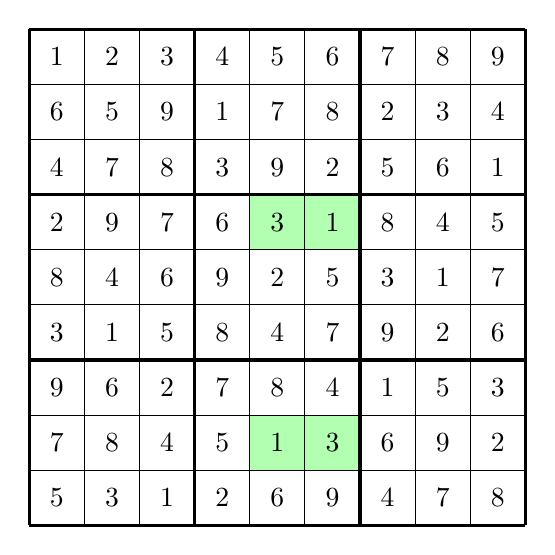
\begin{tikzpicture}
                % Zellgröße
                \def\s{0.7cm}

                % Sudoku-Lösung (kann beliebig angepasst werden)
                \def\sudoku{
                        {1, 2, 3, 4, 5, 6, 7, 8, 9},
                        {6, 5, 9, 1, 7, 8, 2, 3, 4},
                        {4, 7, 8, 3, 9, 2, 5, 6, 1},
                        {2, 9, 7, 6, 3, 1, 8, 4, 5},
                        {8, 4, 6, 9, 2, 5, 3, 1, 7},
                        {3, 1, 5, 8, 4, 7, 9, 2, 6},
                        {9, 6, 2, 7, 8, 4, 1, 5, 3},
                        {7, 8, 4, 5, 1, 3, 6, 9, 2},
                        {5, 3, 1, 2, 6, 9, 4, 7, 8},
                }

                \fill[green!30] (5*\s, 5*\s) rectangle (6*\s, 6*\s);
                \fill[green!30] (4*\s, 5*\s) rectangle (5*\s, 6*\s);

                \fill[green!30] (5*\s, 1*\s) rectangle (6*\s, 2*\s);
                \fill[green!30] (4*\s, 1*\s) rectangle (5*\s, 2*\s);

                % Rasterlinien
                \foreach \x in {0,1,...,9} {
                    \draw[thin] (\x*\s, 0) -- (\x*\s, 9*\s);
                    \draw[thin] (0, \x*\s) -- (9*\s, \x*\s);
                }
                \foreach \x in {0,3,6,9} {
                    \draw[very thick] (\x*\s, 0) -- (\x*\s, 9*\s);
                    \draw[very thick] (0, \x*\s) -- (9*\s, \x*\s);
                }




                % Zahlen eintragen
                \foreach \row [count=\i from 0] in \sudoku {
                    \foreach \num [count=\j from 0] in \row {
                    % Y-Koordinate: Startet oben bei 8.5 und geht pro Zeile 1 runter
                        \node at (\j*\s + 0.5*\s, 8.5*\s - \i*\s) {\num};
                    }
                }
            \end{tikzpicture}
    \end{minipage}
    \caption{Gemeinsame Beschriftung für beide Sudoku-Gitter}
    \label{fig:gemeinsames_sudoku}
\end{figure}

Innerhalb von vollständig ausgefüllten Sudokus kann es Unterquadrate geben.
Ein Beispiel für ein solches Unterquadrat ist in \cref{fig:gemeinsames_sudoku} gegeben.
Ein Unterquadrat besteht aus vier Zellen in denen zwei Ziffern jeweils doppelt vorkommen.
Je zwei Zellen sind dabei in der gleichen Spalte beziehungsweise in der gleichen Zeile.
Entweder beide Zeilen oder beide Spalten sind im gleichen Band.
Durch die Anordnung der Zellen ist es möglich, ein weiteres gültiges Sudoku zu generieren, nur durch Permutieren der beiden Ziffern im Unterquadrat.
Das bedeutet, dass ein partielles Sudoku, welches ein vollständiges Sudoku mit Unterquadrat als Lösung hat, nicht eindeutig lösbar ist,
wenn in keinem der Zellen des Unterquadrats eine Ziffer vorgegeben ist.
Diese Erkenntnis werden wir uns im Backend zu Nutze machen.